\section{リリースについて}
最終成果発表会で得られたレビューをもとに第4サイクルについて改善を行った後、2月頃までのリリースを目標としている。この時期にリリース目標を設定した理由としては、3月に北海道新幹線が開業することが挙げられる。観光客が最も訪れると予想される開業直後に間に合うようリリース準備を進めていく予定だ。今後の作業としては、まずレビューをもとに機能の拡張やUIの再設計を行い、並行して既知のバグの修正を行っていく。これらが完了し次第、App Storeへリリースする。また、リリース後にも定期的なメンテナンスを行っていくほか、季節ごとのコンテンツの追加などの案も検討されている。なお、リリース後のメンテナンスについては、指導教員より最低でも2年間は継続することが望ましいと指導を受けている。
\begin{figure}
	\centering
	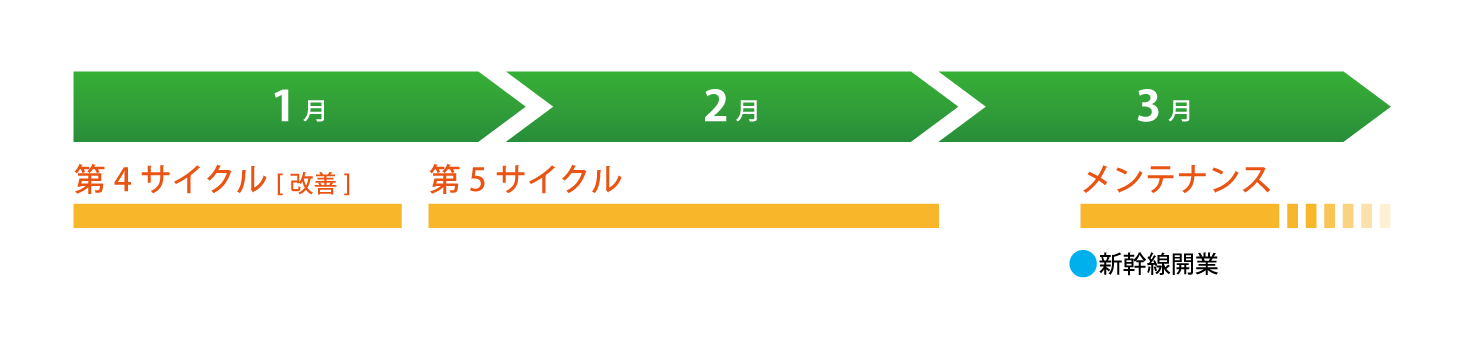
\includegraphics[width=8cm]{release-1.png}
	\caption{今後の予定}
\end{figure}
\bunseki{横山翔栄}